\documentclass[a4paper,10pt,twocolumn]{article}

\usepackage{minted}
\usepackage{algorithm}
\usepackage{verbatim}
\usepackage{graphicx}

\title{Dynamic programming for trajectory optimization with CUDA}
\author{Erik Ward}
\begin{document}
\maketitle

\section{Introduction}

In this report we want to compute optimizal speed profiles
for a vehicle, given an additive cost function, for discrete timesteps
$k=0,..,N$:
$$
c_{0:N} = \sum_{k=0}^{N-1} c(x_k,x_{k+1})
$$
Where $x_k$ is the state of the vehicle at time step $k$, and $N$ the
length of the predction horizion. Here $x_{k+1}$ is a state that 
is reachable from $x_k$ using some valid control input $u_k$.
We assume there is a path,
paramterized by arclength $s$ that we should follow.  The trajectory
of our vehicle is expressed in a path aligned coordinate system and
therfore the state of the vehilce at time step $k$ is given by it's
longitudinal position $s_k$, lateral position $d_k$, and derivates of
these.  In general this problem is non-convex. For example we can have
a situation where another object crosses the path at a range of times,
and we can therfore either accelerate to cross this section before the
other object, or slow down to cross this section after the object.

To solve the problem we will use dynamic programming, where we start
at the end time, $N$, and go backwards in time until we 
find the given start state $x_0$. This is done over a grid of
possible states. 

In this report we provide a proof of concept implementation of 
the dynamic programming problem using CUDA. Our goal is 
not necessarilly solve a problem for an acutal vehicle, rather
we will use a simplified cost function and a relatively course 
grid of states.

\section{Method}

In the following we will assume $d=0$ and instantaneus 
change to different constant accelerations, so the grid will be over
possible longitudinal positions ($s$) and speeds ($v$) for all 
timesteps in the prediction horizion. We will let $N = 10$ and limit the 
speed to be non-negative and at most $35.0 ms^{-1}$. If we start 
our grid at $s=0,v=0$ and have acceleration options:
$a \in \{-2.5,-1.25,0,1.25,2.5\}$ we get $|V|=29$ speed options and $|S|=561$ 
longitudinal position options for each of the $10$ time steps.

\begin{algorithm}
\center
\caption{Serial implementation}
\label{alg:serial}
\begin{footnotesize}
\begin{minted}{c++}
//cost[N-1][:] = 0.0, cost[:N-1][:] = inf
//succ[:][:] = n/a
for(int t=N-1; t>0; --t) {
  for(int v=0; v<V_SZ; ++v) {
    for(int s=0; s<S_SZ; ++s) {
      for(int a=0; a<A_SZ; ++a) {
      
        int curr = get_idx(s,v);
        int prev = get_move(s,v,a);
        float c  = get_cost(prev,curr);

        if(cost[t][curr] + c < cost[t-1][prev]) {
          cost[t-1][prev] = cost[t][curr]+c;
          succ[t-1][prev] = curr_idx;
        }

      }
    }
  }
}
\end{minted}
\end{footnotesize}
\end{algorithm}

Algorithm \ref{alg:serial} shows the serial implementation of 
the dynamic programming algorithm. Here a table of costs and a table 
of successors is filled in, each of size $N\times|S|\times|V|$.
The optimal cost will be stored in the cost table at the inital 
state and the trajctory will be given by the successor table.
For a given speed option at time step $k$, $v_k$, all acceleration options
and possible end positions $s_k$ result in unique $v_{k-1},s_{k-1}$ pairs, and 
therefore the two inner loops can be performed in parallell, for the
$561 \times 5 = 2805$ affected states.

\subsection{Cost function}

Our cost function consists of one term for the deviation with 
respect to a reference speed, and one for the acceleration:
$$
w_v(v_k-v_{ref})^2+w_a a_k^2
$$
We also have a term with infinite cost if the vehicle collides with a
hard coded obstacle occupying positions $s \in [20,30]$ for time step
$t=3$ and a term proportional to a collision probability. For the
collision probability we evalute the probability that we are within
$2.0 m$ of an obstacle with mean position $\mu_s = 40.0$ and with
$\sigma = 2.0$.  This results in two commulative density calculations
for each state.
These terms are ment to emulate typical operations we might want 
to perform when optimizing the cost. 

\section{Implementation}

We implemented the two inner loops of algorithm \ref{alg:serial}
using a simple kernel: \verb|make_move|. A stub is shown in 
Alg. \ref{alg:cuda}.

\begin{algorithm}
\center
\caption{CUDA implementation}
\label{alg:cuda}
\begin{footnotesize}
\begin{minted}{c++}
__global__ 
void make_move(float * const cost,
               int   * const succ,
               int const v,
               int const t,
               move_options const * const move_opt) 
{
    int s = blockIdx.x*blockDim.x  + threadIdx.x;
    int a = blockIdx.y*blockDim.y  + threadIdx.y;
    //...
}
//executed as:
for(int t=N-1; t>0; --t) {
  for(int v=0; v<V_SZ; ++v) {
    make_move<<<grid_dim,block_dim>>>(/*...*/);
  }
}
\end{minted}
\end{footnotesize}
\end{algorithm}


The typical use case for the algorithm would be receeding horizion
planning where we would call the algorithm with different intial 
speeds (and different obstacle configurations), therefore 
we only need to allocate memory once for the \verb|cost| and \verb|succ| arrays, and only need to re-set them before every iteration.
The implementation is available at github: 

\section{Results}

Figure \ref{fig:speed_prof} shows the resulting speed profile when
starting from $v=0.0 ms^{-1}$. 

\begin{figure}
  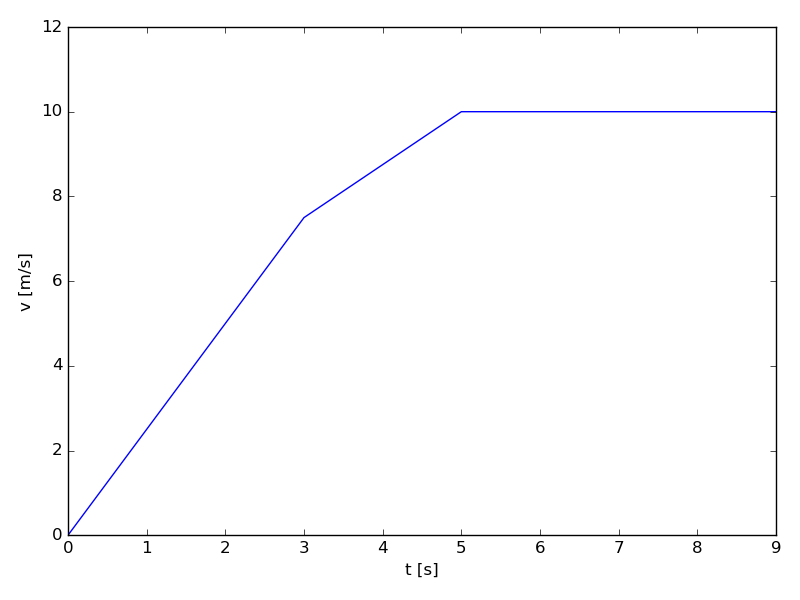
\includegraphics[width=0.9\linewidth]{figure_1.png}
  \caption{Planned speed profile}
  \label{fig:speed_prof}
\end{figure}

To estimate the runtime of both the methods we timed 
memory allocation seprately from execution of the dynamic 
programming algorithm, which was executed 10 times 
for each implementation. Table \ref{tab:runtimes} shows 
the runtimes of the serial version and the CUDA version.
We can observe about a 5.4 times speedup. Also the 
runtime of the GPU version is more consistent, 
with the maximum runtime being only 8\% larger than 
the smallest, compared to the CPU implementation where 
it was 60\% larger.

%MAX runtime cpu: 63.881
%MAX runtime cpu: 39.907

%MAX runtime gpu: 8.283
%MAX runtime gpu: 7.671

\begin{table}
  \center
  \caption{Runtimes}
  \label{tab:runtimes}
  \vspace{0.1cm}
  \begin{tabular}{ c c c}

        & malloc [ms] & mean runtime [ms] \\
    \hline
    CPU & 0.009       & 42.6              \\
    GPU & 254.6       & 7.87
  \end{tabular}
\end{table}

%Starting from v=12.5 m/s v_ref=10
%Malloc data cpu: 0.006 ms 
%MEAN runtime cpu: 42.3268
%Malloc data gpu: 258.008 ms 
%MEAN runtime gpu: 7.902

%Starting from v=0.0  m/s v_ref=10
%Total time for memory alloc on CPU... = 0.009 ms 
%Total time for memory alloc GPU... = 254.595 ms 
%MEAN runtime cpu: 42.5682
%MEAN runtime gpu: 7.8657

\section{Possible extensions}

In this problem we assumed $d=0$ and also instant change of 
acceleration. To improve the generality of the algorithm 
we should include also lateral positions in the state 
grid, as well as accelerations.

Obstacles should not be hard coded, rather a mask for each timestep
should be provided where we check for overlap between the vehicle and
obstacles.  One could also solve a boundary value problem to smooth
out the path of the vehicle between each state, e.g. fit a spline.
Here we should start to see a more drastic improvement of runtimes 
compared to the serial version.

\end{document}

